\newpage
\lecture{10}{Теорема Витали о тонком покрытии.}

\subsection{Лемма и теорема Витали.}

\begin{lemma}[Витали]
    Пусть $\F$~--- семейство невырожденных шаров, причем $\bigcup\F$ ограничено.
    Тогда существует не более чем счётное дизъюнктное семейство $\CG\subset\F$ такое,
    что \[
        \bigcup\F\subset \bigcup_{B\in\CG}\widehat{B},\quad\text{где }
        \widehat{B}_{r}(x):=B_{5r}(x).
    \]
    То есть $\widehat{B}$~--- шар $B$, радиус которого увеличили в 5 раз.

    \begin{proof}

        Пусть шары $B_1,\, \ldots,\, B_{n-1}$ уже построены. Возьмем
        \[
            \F_n:=\{B\in\F:\ B\cap B_i=\varnothing\ \forall i\in\overline{1,\,n-1}\}\quad
            \text{(при $n=1$: $\F_1=\F$)}
        \]
        Пусть также
        \[
            s_n:=\sup\{r(B):\ B\in\F_n\},\quad\text{где $r(B)$~---радиус шара $B$.}
        \]
        Берем $B_n\in\F_n$ так, что $r(B_n)>\dfrac{s_n}{2}$ (если $s_n=0$, то $\F_n=\varnothing$ и
        процесс завершается).

        \begin{figure}[!ht]
            \centering
            

\tikzset{every picture/.style={line width=0.75pt}} %set default line width to 0.75pt        

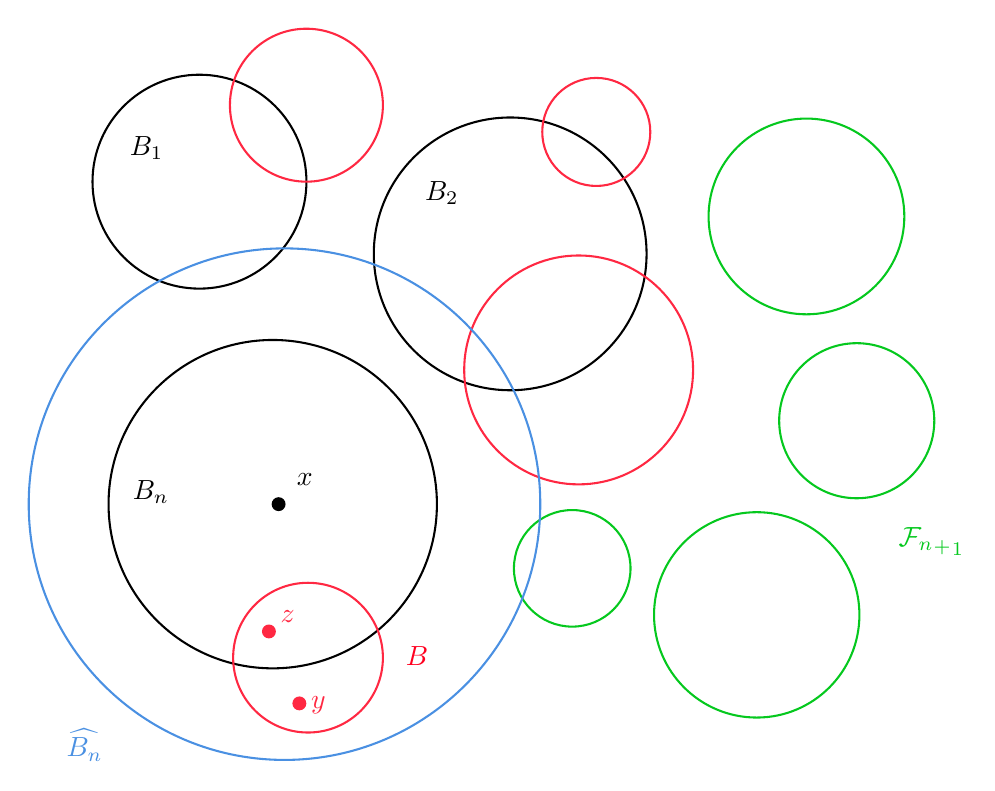
\begin{tikzpicture}[x=1pt,y=1pt,yscale=-1,xscale=1]
%uncomment if require: \path (0,300); %set diagram left start at 0, and has height of 300

%Shape: Ellipse [id:dp25813164220467333] 
\draw   (30.64,63.02) .. controls (30.64,41.67) and (47.94,24.37) .. (69.29,24.37) .. controls (90.63,24.37) and (107.94,41.67) .. (107.94,63.02) .. controls (107.94,84.37) and (90.63,101.67) .. (69.29,101.67) .. controls (47.94,101.67) and (30.64,84.37) .. (30.64,63.02) -- cycle ;
%Shape: Ellipse [id:dp994070922699366] 
\draw   (132.29,89.11) .. controls (132.29,61.89) and (154.35,39.83) .. (181.57,39.83) .. controls (208.78,39.83) and (230.85,61.89) .. (230.85,89.11) .. controls (230.85,116.32) and (208.78,138.39) .. (181.57,138.39) .. controls (154.35,138.39) and (132.29,116.32) .. (132.29,89.11) -- cycle ;
%Shape: Ellipse [id:dp8564778898119749] 
\draw   (36.44,179.55) .. controls (36.44,146.78) and (63,120.22) .. (95.76,120.22) .. controls (128.53,120.22) and (155.09,146.78) .. (155.09,179.55) .. controls (155.09,212.32) and (128.53,238.88) .. (95.76,238.88) .. controls (63,238.88) and (36.44,212.32) .. (36.44,179.55) -- cycle ;
%Shape: Ellipse [id:dp39397600432198776] 
\draw  [color={rgb, 255:red, 255; green, 40; blue, 66 }  ,draw opacity=1 ] (80.3,35.38) .. controls (80.3,20.12) and (92.68,7.75) .. (107.94,7.75) .. controls (123.2,7.75) and (135.57,20.12) .. (135.57,35.38) .. controls (135.57,50.65) and (123.2,63.02) .. (107.94,63.02) .. controls (92.68,63.02) and (80.3,50.65) .. (80.3,35.38) -- cycle ;
%Shape: Ellipse [id:dp55919092603007] 
\draw  [color={rgb, 255:red, 255; green, 40; blue, 66 }  ,draw opacity=1 ] (164.95,131.04) .. controls (164.95,108.2) and (183.46,89.69) .. (206.3,89.69) .. controls (229.14,89.69) and (247.66,108.2) .. (247.66,131.04) .. controls (247.66,153.88) and (229.14,172.4) .. (206.3,172.4) .. controls (183.46,172.4) and (164.95,153.88) .. (164.95,131.04) -- cycle ;
%Shape: Ellipse [id:dp04860568574016577] 
\draw  [color={rgb, 255:red, 255; green, 40; blue, 66 }  ,draw opacity=1 ] (81.46,235.01) .. controls (81.46,220.07) and (93.58,207.96) .. (108.52,207.96) .. controls (123.46,207.96) and (135.57,220.07) .. (135.57,235.01) .. controls (135.57,249.96) and (123.46,262.07) .. (108.52,262.07) .. controls (93.58,262.07) and (81.46,249.96) .. (81.46,235.01) -- cycle ;
%Shape: Ellipse [id:dp36880420423571314] 
\draw  [color={rgb, 255:red, 255; green, 40; blue, 66 }  ,draw opacity=1 ] (193.16,45.05) .. controls (193.16,34.27) and (201.9,25.53) .. (212.68,25.53) .. controls (223.46,25.53) and (232.2,34.27) .. (232.2,45.05) .. controls (232.2,55.83) and (223.46,64.57) .. (212.68,64.57) .. controls (201.9,64.57) and (193.16,55.83) .. (193.16,45.05) -- cycle ;
%Shape: Circle [id:dp4720879733888619] 
\draw  [color={rgb, 255:red, 5; green, 200; blue, 30 }  ,draw opacity=1 ] (182.92,202.74) .. controls (182.92,191.11) and (192.35,181.68) .. (203.98,181.68) .. controls (215.62,181.68) and (225.05,191.11) .. (225.05,202.74) .. controls (225.05,214.37) and (215.62,223.8) .. (203.98,223.8) .. controls (192.35,223.8) and (182.92,214.37) .. (182.92,202.74) -- cycle ;
%Shape: Ellipse [id:dp6697268596924413] 
\draw  [color={rgb, 255:red, 5; green, 200; blue, 30 }  ,draw opacity=1 ] (233.55,219.55) .. controls (233.55,199.06) and (250.16,182.45) .. (270.66,182.45) .. controls (291.15,182.45) and (307.76,199.06) .. (307.76,219.55) .. controls (307.76,240.05) and (291.15,256.66) .. (270.66,256.66) .. controls (250.16,256.66) and (233.55,240.05) .. (233.55,219.55) -- cycle ;
%Shape: Ellipse [id:dp5587771618704152] 
\draw  [color={rgb, 255:red, 5; green, 200; blue, 30 }  ,draw opacity=1 ] (253.26,75.58) .. controls (253.26,56.05) and (269.1,40.22) .. (288.63,40.22) .. controls (308.16,40.22) and (323.99,56.05) .. (323.99,75.58) .. controls (323.99,95.11) and (308.16,110.95) .. (288.63,110.95) .. controls (269.1,110.95) and (253.26,95.11) .. (253.26,75.58) -- cycle ;
%Shape: Ellipse [id:dp6282906387242082] 
\draw  [color={rgb, 255:red, 5; green, 200; blue, 30 }  ,draw opacity=1 ] (278.77,149.4) .. controls (278.77,133.93) and (291.32,121.38) .. (306.79,121.38) .. controls (322.27,121.38) and (334.82,133.93) .. (334.82,149.4) .. controls (334.82,164.88) and (322.27,177.42) .. (306.79,177.42) .. controls (291.32,177.42) and (278.77,164.88) .. (278.77,149.4) -- cycle ;
%Flowchart: Connector [id:dp35662527833016466] 
\draw  [fill={rgb, 255:red, 0; green, 0; blue, 0 }  ,fill opacity=1 ] (95.76,179.55) .. controls (95.76,180.72) and (96.72,181.68) .. (97.89,181.68) .. controls (99.06,181.68) and (100.02,180.72) .. (100.02,179.55) .. controls (100.02,178.38) and (99.06,177.42) .. (97.89,177.42) .. controls (96.72,177.42) and (95.76,178.38) .. (95.76,179.55) -- cycle ;
%Shape: Ellipse [id:dp6938349115010671] 
\draw  [color={rgb, 255:red, 74; green, 144; blue, 226 }  ,draw opacity=1 ] (7.59,179.55) .. controls (7.59,128.51) and (48.97,87.13) .. (100.02,87.13) .. controls (151.06,87.13) and (192.44,128.51) .. (192.44,179.55) .. controls (192.44,230.59) and (151.06,271.97) .. (100.02,271.97) .. controls (48.97,271.97) and (7.59,230.59) .. (7.59,179.55) -- cycle ;
%Flowchart: Connector [id:dp6565155031810235] 
\draw  [color={rgb, 255:red, 255; green, 40; blue, 66 }  ,draw opacity=1 ][fill={rgb, 255:red, 255; green, 40; blue, 66 }  ,fill opacity=1 ] (92.26,225.55) .. controls (92.26,226.72) and (93.22,227.68) .. (94.39,227.68) .. controls (95.56,227.68) and (96.52,226.72) .. (96.52,225.55) .. controls (96.52,224.38) and (95.56,223.42) .. (94.39,223.42) .. controls (93.22,223.42) and (92.26,224.38) .. (92.26,225.55) -- cycle ;
%Flowchart: Connector [id:dp7973879357254914] 
\draw  [color={rgb, 255:red, 255; green, 40; blue, 66 }  ,draw opacity=1 ][fill={rgb, 255:red, 255; green, 40; blue, 66 }  ,fill opacity=1 ] (103.26,251.55) .. controls (103.26,252.72) and (104.22,253.68) .. (105.39,253.68) .. controls (106.56,253.68) and (107.52,252.72) .. (107.52,251.55) .. controls (107.52,250.38) and (106.56,249.42) .. (105.39,249.42) .. controls (104.22,249.42) and (103.26,250.38) .. (103.26,251.55) -- cycle ;

% Text Node
\draw (43.06,45.52) node [anchor=north west][inner sep=0.75pt]   [align=left] {$\displaystyle B_{1}$};
% Text Node
\draw (149.73,61.75) node [anchor=north west][inner sep=0.75pt]   [align=left] {$\displaystyle B_{2}$};
% Text Node
\draw (44.1,169.97) node [anchor=north west][inner sep=0.75pt]   [align=left] {$\displaystyle B_{n}$};
% Text Node
\draw (320.81,186.98) node [anchor=north west][inner sep=0.75pt]  [color={rgb, 255:red, 5; green, 200; blue, 30 }  ,opacity=1 ] [align=left] {$\displaystyle {{\mathcal{F}_{n}}_{+}}_{1}$};
% Text Node
\draw (142.72,229.88) node [anchor=north west][inner sep=0.75pt]  [color={rgb, 255:red, 255; green, 0; blue, 31 }  ,opacity=1 ] [align=left] {$\displaystyle B$};
% Text Node
\draw (103.35,167.33) node [anchor=north west][inner sep=0.75pt]   [align=left] {$\displaystyle x$};
% Text Node
\draw (20.14,259.73) node [anchor=north west][inner sep=0.75pt]  [color={rgb, 255:red, 74; green, 144; blue, 226 }  ,opacity=1 ] [align=left] {$\displaystyle \widehat{B_{n}}$};
% Text Node
\draw (97.5,217) node [anchor=north west][inner sep=0.75pt]  [color={rgb, 255:red, 255; green, 40; blue, 66 }  ,opacity=1 ] [align=left] {$\displaystyle z$};
% Text Node
\draw (108.5,248) node [anchor=north west][inner sep=0.75pt]  [color={rgb, 255:red, 255; green, 40; blue, 66 }  ,opacity=1 ] [align=left] {$\displaystyle y$};


\end{tikzpicture}
            \caption{К лемме Витали.}
            \label{fig:balls}
        \end{figure}

        На рисунке \ref{fig:balls} черным указаны шары, которые выбраны, красным~--- шары, которые пересекаются с
        выбранными
        (их мы не берем в $\F_{n+1}$) и зеленым~--- шары, которые составляют $\F_{n+1}$.
        Рассмотрим некоторый шар $B\in\F_n$, который пересекается с $B_n$.
        Раздуем шар $B_n$ в пять раз, то есть рассмотрим $\widehat{B}_n$ (на рисунке синий цвет).
        Утверждается, что раздутый шар покроет шар $B$. В самом деле пусть $x$~--- центр $B_n$,
        $z\in B\cap B_n$ и $y\in B$. Тогда по неравенству треугольника имеем \[
            |x-y|\leqslant|x-z|+|z-y|\leqslant r(B_n)+2r(B).
        \]
        Оценим $r(B)$:
        \[
            B\in\F_n\Rightarrow r(B)\leqslant\sup_{B\in\F_n} r(B)=s_n<2r(B_n).
        \]
        То есть,
        \[
            |x-y|\leqslant r(B_n)+2r(B)<5r(B_n)\Rightarrow B\subset \widehat{B}_n.
        \]

        Итак, если процесс завершился за конечное число шагов, то новые раздутые шары покрывают все исходные.

        Пусть теперь процесс не завершается за конечное число шагов.
        По построению $\bigsqcup\limits_{n=1}^{\infty}B_n\subset \bigcup\F\subset B_{R}(0)$, где
        $R>0$~--- достаточно большая константа, она существует, так как $\bigcup\F$ ограничено по условию.

        Тогда имеем,
        \[
            \lambda\left(\bigsqcup_{n=1}^{\infty}B_n\right)\leqslant\lambda(B_{R}(0))<\infty.
        \]
        Но
        \[
            \lambda\left(\bigsqcup_{n=1}^{\infty}B_n\right)=
            \sum_{n=1}^{\infty}\lambda(B_n).
        \]
        Значит ряд сходится, следовательно $\lambda(B_n)\xrightarrow[n\to\infty]{}0$, но тогда
        и $r(B_n)\xrightarrow[n\to\infty]{}0$.

        Тогда $\forall B\in\F\ r(B)>0\Rightarrow s_n<r(B)$ при достаточно большом $n$. Поэтому при таких $n$
        $B\notin\F_n$.

        Выберем наименьшее $n$ так, что $B\notin\F_{n+1}$.
        Тогда $B\in\F_n\Rightarrow B\in\F_n\setminus\F_{n+1}$, то есть $B$ <<удаляется>> на
        $n$"=ом шаге, поэтому $B\cap B_n=\varnothing$. По доказанному выше получаем, что
        $B\subset \widehat{B}_n$. Итак,
        \[
            \forall B\in\F\quad\exists n:\ B\subset \widehat{B}_n\Rightarrow\bigcup\F\subset
            \bigcup_{B\in\CG}\widehat{B}.
        \]

    \end{proof}
\end{lemma}

Далее докажем более сильное утверждение, но сначала дадим определение.
\begin{definition}
    Семейство $\F$ невырожденных замкнутых шаров будем называть \mdef{тонким покрытием}
    множества $A\subset\R^d$, если \[
        \forall x\in A\quad \forall\varepsilon>0\quad \exists B\in\F:\: x\in B
        ,\quad r(B)<\varepsilon.
    \]
\end{definition}

\begin{theorem}[Витали, о тонком покрытии]
    Пусть $\F$~--- тонкое покрытие $A\subset\R^d$. Тогда существует дизъюнктное
    не более чем счетное семейство $\CG\subset\F$ такое, что \[
        \lambda\left(A\setminus\bigsqcup_{B\in\CG}B\right)=0.
    \]

    \begin{proof}

        Докажем для случая ограниченного $A$ (случай неограниченного $A$ сводится к этому~--- разрезаем $A$ на
        счетное число ограниченных множеств и аккуратно покрываем их).

        Выкинем из $\F$ шары, радиусы которых больше 1, а также шары, не пересекающие $A$.
        Оставшееся семейство по-прежнему будет
        тонким покрытием $A$ и при этом $\bigcup\F$ ограничено.

        Построим семейство $\CG=\{B_n\}_{n=1}^{\infty}\subset\F$ так же, как в доказательстве
        леммы Витали.

        \begin{center}
            \tikzset{every picture/.style={line width=0.75pt}} %set default line width to 0.75pt        

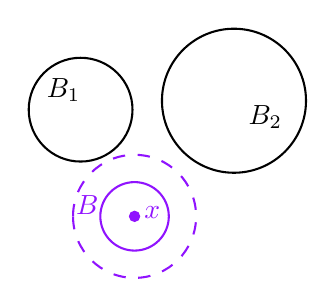
\begin{tikzpicture}[x=0.75pt,y=0.75pt,yscale=-1,xscale=1]
%uncomment if require: \path (0,300); %set diagram left start at 0, and has height of 300

%Shape: Circle [id:dp08395379661992064] 
\draw   (40,89) .. controls (40,75.19) and (51.19,64) .. (65,64) .. controls (78.81,64) and (90,75.19) .. (90,89) .. controls (90,102.81) and (78.81,114) .. (65,114) .. controls (51.19,114) and (40,102.81) .. (40,89) -- cycle ;
%Shape: Circle [id:dp003534917885936295] 
\draw   (104.2,84.7) .. controls (104.2,65.54) and (119.74,50) .. (138.9,50) .. controls (158.06,50) and (173.6,65.54) .. (173.6,84.7) .. controls (173.6,103.86) and (158.06,119.4) .. (138.9,119.4) .. controls (119.74,119.4) and (104.2,103.86) .. (104.2,84.7) -- cycle ;
%Flowchart: Connector [id:dp6639375115419266] 
\draw  [color={rgb, 255:red, 144; green, 19; blue, 254 }  ,draw opacity=1 ][fill={rgb, 255:red, 144; green, 19; blue, 254 }  ,fill opacity=1 ] (93.2,140.4) .. controls (93.2,139.18) and (92.22,138.2) .. (91,138.2) .. controls (89.78,138.2) and (88.8,139.18) .. (88.8,140.4) .. controls (88.8,141.62) and (89.78,142.6) .. (91,142.6) .. controls (92.22,142.6) and (93.2,141.62) .. (93.2,140.4) -- cycle ;
%Shape: Circle [id:dp10935286037474001] 
\draw  [color={rgb, 255:red, 144; green, 19; blue, 254 }  ,draw opacity=1 ][dash pattern={on 4.5pt off 4.5pt}] (61.35,140.4) .. controls (61.35,124.02) and (74.62,110.75) .. (91,110.75) .. controls (107.38,110.75) and (120.65,124.02) .. (120.65,140.4) .. controls (120.65,156.78) and (107.38,170.05) .. (91,170.05) .. controls (74.62,170.05) and (61.35,156.78) .. (61.35,140.4) -- cycle ;
%Shape: Circle [id:dp5911363270914514] 
\draw  [color={rgb, 255:red, 144; green, 19; blue, 254 }  ,draw opacity=1 ] (74.5,140.4) .. controls (74.5,131.29) and (81.89,123.9) .. (91,123.9) .. controls (100.11,123.9) and (107.5,131.29) .. (107.5,140.4) .. controls (107.5,149.51) and (100.11,156.9) .. (91,156.9) .. controls (81.89,156.9) and (74.5,149.51) .. (74.5,140.4) -- cycle ;

% Text Node
\draw (94.2,134.2) node [anchor=north west][inner sep=0.75pt]  [color={rgb, 255:red, 144; green, 19; blue, 254 }  ,opacity=1 ] [align=left] {$\displaystyle x$};
% Text Node
\draw (61.4,129) node [anchor=north west][inner sep=0.75pt]  [color={rgb, 255:red, 144; green, 19; blue, 254 }  ,opacity=1 ] [align=left] {$\displaystyle B$};
% Text Node
\draw (47.2,72.6) node [anchor=north west][inner sep=0.75pt]   [align=left] {$\displaystyle B_{1}$};
% Text Node
\draw (144.4,85.4) node [anchor=north west][inner sep=0.75pt]   [align=left] {$\displaystyle B_{2}$};


\end{tikzpicture}

        \end{center}

        Рассмотрим $x$, которое не принадлежит объединению первых $n$ шаров: \[
            x\notin \underbrace{\bigcup\limits_{k=1}^n B_k}_{\text{замкнуто}}\Rightarrow
            \rho\left(x,\, \bigcup_{k=1}^n B_k\right)>0\Rightarrow\exists B\in\F:\ x\in B,\,
            B\cap\bigcup_{k=1}^nB_k=\varnothing.
        \]

        Как было показано в доказательстве леммы Витали:
        \[
            \exists! m\in\N:\quad B\in\F_{m}\setminus\F_{m+1}.
        \]
        С другой стороны,
        \[
            B\in\bigcap_{k=1}^n\F_k\Rightarrow m>n.
        \]
        Так как $B\cap B_m\Rightarrow B\subset \widehat{B}_m$, то получаем
        \[
            x\in\bigcup_{k=n+1}^{\infty}\widehat{B}_k.
        \]

        То есть доказано следующее утверждение:
        \begin{equation}
            \label{eq:lect10:vit}
            \boxed{A\setminus\bigsqcup_{k=1}^{\infty} B_k\subset
                \bigcap_{n=1}^{\infty}\bigcup_{k=n+1}^{\infty}\widehat{B}_k}
        \end{equation}
        В самом деле,
        \[
            x\in A\setminus\bigsqcup_{k=1}^{\infty}B_k\Rightarrow\forall n\quad
            x\in A\setminus\bigsqcup_{k=1}^{n}B_k.
        \]
        А также
        \[
            A\setminus\bigsqcup_{k=1}^{n}B_k\subset \bigcup_{k=n+1}^{\infty}\widehat{B}_k.
        \]

        Перейдем к мере Лебега в уравнении \eqref{eq:lect10:vit}:
        \[
            \forall n\in\N \quad \lambda^*\left(A\setminus\bigsqcup_{k=1}^{\infty}B_k\right)
            \leqslant\lambda^*\left(\bigcup_{k=n+1}^{\infty}\widehat{B}_k\right)
            \leqslant\sum_{k=n+1}^{\infty}\lambda^*\left(\widehat{B}_k\right)
            =\sum_{k=n+1}^{\infty}5^d\lambda(B_k).
        \]
        Поскольку шары дизъюнктны и лежат в ограниченном множестве можно записать:
        \[
            \sum_{k=1}^{\infty}\lambda(B_k)<\infty\Rightarrow\lim_{n\to\infty}
            \sum_{k=n+1}^{\infty}\lambda(B_k)=0.
        \]
        Итак,
        \[
            \forall \varepsilon>0\quad \lambda^*\left(A\setminus\bigsqcup_{k=1}^{\infty}B_k\right)<
            \varepsilon\Rightarrow\lambda^*\left(A\setminus\bigsqcup_{k=1}^{\infty}B_k\right)=0.
        \]

    \end{proof}
\end{theorem}

\subsection{Точки Лебега.}

\begin{definition}
    Пусть $A\subset\R^d$ измеримо по Лебегу. Обозначим
    \[
        L_A:=\left\{x\in\R^d:\quad \exists\lim_{r\to n}\dfrac{\lambda\left(A\cap B_r(x)
            \right)}{\lambda(B_r(x))}=1\right\}.
    \]
    Точка $x\in\R^d$ называется \mdef{точкой Лебега} множества $A$ тогда и только тогда, когда
    $x\in L_A$.

    \begin{remark}
        Точки, не принадлежащие $A$, могут лежать в $L_A$. Более того, можно заметить, что
        \[
            L_{A^C}=\left\{x\in\R^d:\quad \exists\lim_{r\to n}\dfrac{\lambda\left(A\cap B_r(x)
                \right)}{\lambda(B_r(x))}=0\right\}.
        \]
    \end{remark}
\end{definition}

\begin{theorem}
    Если $A\subset\R^d$ измеримо по Лебегу, то \textit{почти все}
    $x\in A$ являются точками Лебега множества $A$, то есть
    \[
        \exists N\subset A:\quad \lambda^*(N)=0:\quad \forall x\in A\setminus N\text{~---
            точка Лебега множества $A$.}
    \]

    \begin{next0}
        \[
            \lambda(A\triangle L_A)=0.
        \]
    \end{next0}

    \begin{proof}

        Докажем вначале для случая, когда $A$ ограничено. Заметим, что
        \[
            x\in L_A\Leftrightarrow \lim_{\overline{r\to0}}\dfrac{\lambda(A\cap B_r(x))}
            {\lambda(B_r(x))}=1.
        \]
        Введем множество <<плохих>> точек:
        \[
            N_{\alpha}:=\left\{x\in A:\quad \lim_{\overline{r\to0}}\dfrac{\lambda(A\cap B_r(x))}
            {\lambda(B_r(x))}\leqslant\alpha\right\},\text{ где } \alpha\in(0,\, 1).
        \]

        Докажем, что $\forall\alpha\in(0,\,1)$ мера $N_{\alpha}$ равна нулю.
        В силу внешней регулярности меры Лебега
        \[
            \forall \varepsilon>0\quad\exists\text{открытое }U\supset N_{\alpha}:\quad
            \lambda(U)<\lambda^*(N_{\alpha})+\varepsilon.
        \]

        Из определения множества $N_{\alpha}$ следует, что: \[
            \exists\{r_n\to 0\}:\quad \dfrac{\lambda(A\cap B_{r_n}(x))}{\lambda(B_{r_n}(x))}\leqslant\alpha.
        \]

        Рассмотрим тогда
        \[
            \F=\left\{\overline{B}_{r_n(x)}(x)\ \mid\ x\in N_{\alpha},\, n\in\N\text{ такие, что }
            \overline{B}_{r_n(x)}(x)\subset U\right\}.
        \]
        Понятно, что $\F$~--- тонкое покрытие множества $A$.

        По теореме Витали существует дизъюнктное не более чем счетное семейство
        $\CG\subset \F$:
        \[
            \lambda\left(N_{\alpha}\setminus\bigsqcup_{B\in\CG}B\right)=0.
        \]
        Тогда \begin{align*}
            \lambda^*(N_{\alpha}) & \leqslant\lambda^*\left(N_{\alpha}\cap
            \bigsqcup_{B\in\CG}B\right)+\underbrace{\lambda^*\left(
                N_{\alpha}\setminus\bigsqcup_{B\in\CG}B\right)}_{0}\leqslant
            \sum_{B\in\CG}\lambda^*(N_{\alpha}\cap B)\leqslant                                              \\
                                  & \leqslant[N_{\alpha}\subset A]\leqslant\sum_{B\in\CG}\lambda^*(A\cap B)
            \leqslant\sum_{B\in\CG}\alpha\lambda(B)=\alpha\lambda\left(\bigsqcup
            _{B\in\CG}B\right)\leqslant\alpha\lambda(U).
        \end{align*}
        Итак, 
        \[
            \lambda^*(N_{\alpha})\leqslant\alpha\lambda(U)<\alpha\left(\lambda^*(N_{\alpha})+
            \varepsilon\right)\Rightarrow (1-\alpha)\lambda^*(N_{\alpha})<\alpha\varepsilon.
        \]
        Откуда в силу произвольности $\varepsilon$ следует, что $\lambda^*(N_{\alpha})=0$.

        Осталось заметить, что если $x$~--- не точка Лебега, то 
        \[
            \lim_{\overline{r\to 0}}\dfrac{\lambda(A\cap B_r(x))}{\lambda(B_r(x))}<1
            \Rightarrow\exists\alpha\in(0,\, 1)\cap\Q:\quad
            \lim_{\overline{r\to 0}}\dfrac{\lambda(A\cap B_r(x))}{\lambda(B_r(x))}<\alpha
            \Leftrightarrow x\in N_{\alpha}.
        \]
        Тогда \[
            A\setminus L_A\subset \bigcup_{\alpha\in(0,\,1)\cap \Q}N_{\alpha}\text{~---
            счетное объединение множеств меры нуль}.
        \]
        Откуда, окончательно, $\lambda(A\setminus L_A)=0$.

        Пусть теперь $A$~--- неограниченно. Представим $A$ в виде 
        \[
            A = \bigcup_{n=1}^{\infty}A\cap B_{n}(0).    
        \] 
        Известно, что $\forall n\in \N$ почти все $x\in A\cap B_{n}(0)$ являются
        точками Лебега множества $A\cap B_n(0)$, а значит и множества $A$.
        Обозначим $N_n\subset A\cap B_n(0)$~--- те $x\in A\cap B_{n}(0)$, 
        которые не являются точками Лебега. Тогда $N_n$ покрывает множество 
        тех точек $x\in B_n$, которые не являются точками Лебега множества $A$.

        Тогда множество тех точек, которые не являются точками Лебега множества $A$ имеет меру нуль:
        \[
            A\setminus L_A\subset \underbrace{\bigcup_{n=1}^{\infty}N_n}_{\lambda=0}.
        \]

    \end{proof}
\end{theorem}